%--------------------------------------------------------------------------
% Literature Review
%--------------------------------------------------------------------------

\chapter{Literature Review}
\label{cha: literature-review}

\section{Synthetic aperture radar for forest applications}
\label{sec: litrev-sar-forest-apps}

Synthetic aperture radar (SAR) is a viable alternative to optical remote sensing for land cover characterisation, mapping, and monitoring to support environmental studies and resource management. SAR systems transmit short pulses of microwave energy toward the Earth’s surface, which then interact with different surface features like vegetation, infrastructure, and water bodies, and the sensor provides information such as backscattering coefficients, which represent the strength of the microwave energy emitted from the antenna and returned after scattering by the target features (\cite{thapa_evaluation_2014}). Backscatter is characterised by polarised modes of the transmitted and received signals, particularly the co-polarisation channels: horizontal transmit and horizontal receive (HH) and vertical transmit and vertical receive (VV); and the cross-polarisation channels: horizontal transmit and vertical receive (HV) and vertical transmit and horizontal receive (VH). Scattering mechanisms that contribute to backscattered energy include surface scattering from water bodies and slightly rough surfaces, double bounce scattering from dihedral surfaces and edges, and volume scattering from forests and other vegetation (\cite{van_zyl_unsupervised_1989}; \cite{freeman_three-component_1998}).

SAR sensors are unaffected by atmospheric conditions and can penetrate through clouds, haze, and smoke, thereby overcoming limitations of optical data in cloudy tropical regions (\cite{achard_estimating_2010}; \cite{shimada_generating_2010}). As an active remote sensing system, radar imagery can be calibrated to a very high degree of accuracy with its constant illumination geometry and well-established transmit/receive power spectra; hence allowing the comparison of backscatter values ($\sigma$\textsuperscript{0}) over time and space (i.e., structurally and electrically similar vegetation have the same backscattering behaviour anywhere on earth; \cite{kellndorfer_toward_1998}). SAR data can be acquired consistently on a repetitive basis regardless of weather conditions; hence, these data can potentially be used to complement or replace optical remote sensing systems in an operational programme for mapping and monitoring of forests (\cite{almeida-filho_detecting_2007}).

Notable studies, as described next, were aimed at understanding the relationships between SAR data and forest structure to explore the utility of SAR for forest applications. Ulaby et al. (\citeyearpar{ulaby_textural_1986}) studied the suitability of radar data from two L-band SAR missions, Seasat and the Shuttle Imaging Radar (SIR-A), for mapping forest types in North and South America. They found that combining backscatter and texture measures improved discrimination of forest types using supervised classification techniques. Durden et al. (\citeyearpar{durden_modeling_1989}) described a theoretical scattering mechanism model for forested areas and found good agreement between modelled polarisation signatures with observed polarisation measurements using ground data and AIRSAR L-band data. Le Toan (\citeyearpar{le_toan_relating_1992}) analysed the relationships of multi-frequency (i.e., C, L, and P bands) quad-polarimetric (i.e., HH, HV, VH, VV) AIRSAR data with forest stand parameters measured from pine forests ranging from young to mature stages, which revealed that longer wavelength SAR data, particularly P- and L-bands, had strong correlations and high sensitivities to forest biomass. Moreover, cross-polarised signals showed high correlations with forest stand parameters. Imhoff (\citeyearpar{imhoff_theoretical_1995}) investigated the effect of forest structural differences in equal-biomass broadleaf forest stands on radar backscatter similarly from multi-frequency quad-polarimetric AIRSAR data. The results indicated that structure exerted a substantial effect on backscatter, which tended to increase with forest structural consolidation into fewer and larger parts; hence providing a structural link to positive correlations of radar backscatter with aboveground biomass. Woodhouse et al. (\citeyearpar{woodhouse_radar_2012}) believes that \enquote{radar is typically the best satellite-based remote sensing tool for mapping forest extent, estimating forest structural variability, and detecting deforestation and degradation.}

The Advanced Land Observing Satellite (ALOS), launched on 24 January 2006, was developed for detailed observation of the Earth’s surface and frequent monitoring of global environmental changes, such as forest ecosystems, using both optical and SAR sensors (\cite{shimada_advanced_2010}). Onboard ALOS is the Phased Array type L-band Synthetic Aperture Radar (PALSAR), a multi-polarisation L-band SAR system, which builds on the experience gained from its predecessor, the Japan Earth Resources Satellite (JERS-1), similarly a spaceborne L-band SAR sensor that was successfully used for global rainforest and boreal forest mapping projects in the 1990s (\cite{rosenqvist_global_2000}; \cite{rosenqvist_overview_2004}). L-band SAR (\url{~}25 cm wavelength) is particularly useful in mapping forest areas due to its longer wavelengths and shorter frequencies (\cite{thapa_evaluation_2014}), which in turn allows greater penetration through forest vegetation by the transmitted signal and sensitivity for detecting deforestation (i.e., L-band backscatter is typically lower in non-forest areas compared to forests) and forest inundation (i.e., L-band backscatter is typically lower in inundated forest areas); thereby yielding important information for forest cover monitoring (\cite{shimada_advanced_2010}; \cite{shimada_generating_2010}). The co-polarised channel (i.e., HH) has been found to be sensitive to vertical structure, such as regrowth in clear-cut regions, while the cross-polarised channel (i.e., HV) is less sensitive to vertical structure in low vegetation or clear-cut areas (\cite{shimada_advanced_2010}). ALOS also featured a unique systematic observation strategy to provide consistent, semi-annual, wall-to-wall observations at fine spatial resolution of the Earth's entire landmass during the satellite's lifetime (\cite{rosenqvist_alos_2007}).

Since its launch, ALOS/PALSAR data have been used for various forest applications such as detecting tropical deforestation (\cite{almeidafilho_using_2009}; \cite{rahman_mapping_2010}; \cite{whittle_detection_2012}; \cite{motohka_using_2014}); time-series mapping of forest cover (\cite{thapa_tropical_2013}; \cite{shimada_new_2014}); assessing forest fragmentation (\cite{dong_50-m_2014}); estimating mangrove biomass (\cite{hamdan_l-band_2014}) and forest aboveground biomass (\cite{mitchard_using_2009}; \cite{morel_estimating_2011}; \cite{sarker_potential_2012}; \cite{cartus_mapping_2012}; \cite{rahman_retrieval_2013}; \cite{mermoz_decrease_2015}; \cite{thapa_potential_2015}); mapping mangrove areas (\cite{rocha_de_souza_pereira_mapping_2012}) and changes in mangrove extent (\cite{nascimento_mapping_2013}); and assessing processes of forest disturbances and successional dynamics (\cite{joshi_mapping_2015}; \cite{mermoz_forest_2016}). PALSAR is also one of the main data sources for the Task on Forest Carbon Tracking, established by the Group on Earth Observation in 2009 as a global forest monitoring system in support to the United Nations Framework Convention on Climate Change post-Kyoto Protocol framework (\cite{shimada_advanced_2010}).

\section{Land and forest cover type mapping using\\ ALOS/PALSAR}
\label{sec: litrev-forest-mapping-palsar}

Studies have demonstrated the use of ALOS/PALSAR for mapping tropical forest types and broad land cover categories, which is the topic of interest of this study. For example, quad-polarimetric PALSAR data were used for mapping broad land cover categories. Rahman and Sumantyo \citeyearpar{rahman_mapping_2010} mapped forest, forest re-growth, upland soil/shrub, lowland soil, settlement, and water/wetlands in Southern Chittagong, Bangladesh. They found that forests were discriminated well from other land cover categories, although forest re-growth was not detected, and only a 66\% overall classification accuracy was achieved. Mishra et al. \citeyearpar{mishra_land_2011} tested different classifiers for mapping broad land cover types (i.e., tall vegetation, short vegetation, urban, bare soil, and water) in Roorkee, India. Their results showed that decision tree classifier obtained an 86\% overall accuracy and performed better than other classification techniques. Avtar et al. \citeyearpar{avtar_characterization_2012} assessed two images for characterising forest types (evergreen, deciduous, sparsely deciduous) and deforestation in Northern Cambodia. Their study showed that HV-polarised backscatter coefficient, cross-polarisation ratio (HH/HV), among other parameters gave better results for characterising forest types. Further, they observed that HV-polarised backscatter coefficient of evergreen forest was higher compared to deciduous and sparsely deciduous forest types, particularly due to the multiple canopies of evergreen forests that enhance volume scattering.

Previous studies have used dual-polarised PALSAR data combined with texture information derived from the radar images. Longépé et al. \citeyearpar{longepe_assessment_2011} mapped land cover types (i.e., dry forest, wet forest, acacia, clear cut, oil palm, others) in Riau province, Sumatra, Indonesia using dual-polarised (HH, HV) PALSAR data and texture measures. The overall agreement with reference data was \url{~}70\% for land cover classification and \url{~}87\% for natural forest discrimination. Similarly, Rakwatin et al. \citeyearpar{rakwatin_using_2012} mapped broad land cover types (i.e., forest, oil palm, acacia, clear cut, water) in Riau province, Indonesia, and reported a 73\% overall classification accuracy. The overall accuracies for land cover classification increased by about 10\% when combined with texture information. Li et al. \citeyearpar{li_comparative_2012} used dual-polarised PALSAR data and texture measures for mapping broad land cover types (i.e., forest, succession, agropasture, water, wetland, urban) in Altamira, Para, Brazil. The best classification resulted in a 74\% overall accuracy, of which textural information was valuable for improving vegetation classification. They also reported difficulties in discriminating between forest classes and between forest succession classes.

Discriminating tropical forest types based on successional stages have been studied due to its importance in understanding the role of forest regeneration in global carbon cycles. Li et al. \citeyearpar{li_comparative_2012} found that neither L-band PALSAR nor C-band RADARSAT-2 dual-polarisation data can accurately separate between detailed forest types (upland, flooding, liana) and between forest succession stages (initial, intermediate, advanced). Upon testing different classifiers, they also found that no algorithm could successfully separate forest succession stages. Liesenberg \& Gloaguen \citeyearpar{liesenberg_evaluating_2013} evaluated different PALSAR data modes (e.g., single-, dual-, quad-polarimetric, and interferometric) to characterize and classify primary, successional secondary, and riparian forest classes in Eastern Amazon, Brazil. They found that while quad-polarised data provided better results compared to single or dual-polarised data, the overall accuracies remained low. Radar backscatter of primary and riparian forests were higher than those observed for successional secondary forest types (initial, intermediate, advanced). Backscatter values tended to increase from advanced to initial secondary stage forest, although no substantial differences were observed between successional secondary forest types.

\section{Forest classification systems}
\label{sec: litrev-forest-class-system}

\subsection{FAO Global Forest Resources Assessment forest classification}

The above examples on mapping forest cover types using ALOS/PALSAR data have adopted classification schemes based on forest age or successional stages (e.g., primary, secondary), disturbance gradients (e.g., pristine, degraded), or on bespoke classes suited to the area of interest. However, using different classification schemes makes compatibility between datasets difficult to ascertain and hinders the comparative analysis of land cover types across space and time in a consistent manner (\cite{ahlqvist_search_2008}). Although, at present, no definitive universally accepted land cover classification system exists (Townshend et al., 2010), such a classification system is crucial for the evaluation, comparison, and change analysis of land cover products (\cite{giri_brief_2012}).

The Global Forest Resources Assessments (GFRA), coordinated by FAO at the request of its member countries, provides periodic information on the situation of the world's forests to support decision-making in investment and policymaking in forestry and sustainable development (\cite{fao_global_2015}). One of the primary sources of data for these assessments is the Country Report prepared by national correspondents, which are based on National Forest Assessments (NFA) and are submitted to FAO for consolidation in a global report produced every 5 years. Forest inventories, which are based on systematic field sampling and complemented by remote sensing, are the primary means for data collection within these NFAs. The FAO formulates guidelines for country reporting, including forest classification terms and definitions, to ensure compatibility and interoperability of information across countries and time for global forest resources monitoring, as well as facilitating comparative analysis of land cover change within national-level assessments.

In the Philippines, national remote sensing surveys were conducted by NAMRIA to complement national forest inventories for the reporting periods in 2005 and 2010 (i.e., 2003 and 2010 land cover map products), which adopted the FAO GFRA classification and definitions (Table \ref{tab: intro-table2.1}). Forest inventories were only implemented for the 2005 reporting, but were not carried out for the 2010 reporting (\cite{fao_2010_2010}). For consistency, this study similarly adopted the same forest classification system for evaluating L-band PALSAR data for distinguishing forest cover types based on this system, which would allow comparison with the official land cover maps.\\

\begin{spacing}{1.0}
\begin{longtable}[h!]{ p{3.5cm} p{10.5cm} }

    \caption[Global Forest Resources Assessment categories and definitions.]{Categories and definitions based on the Global Forest Resources Assessment (Source: \cite{fao_2005_2005}; \cite{fao_2010_2010}).}
    \label{tab: intro-table2.1}\\
    
    \toprule
    Category & Definition \\
    \midrule
    \endhead

    Forest & Land with tree crown cover (or equivalent stocking level) of more than 10\% and area of more than 0.5 ha. \\[5pt]
    Broadleaved forest & Forest with predominance (more than 75\% of tree crown cover) of trees of broadleaved species.\\[5pt]
    Coniferous forest & Forest with predominance (more than 75\% of tree crown cover) of trees of coniferous species.\\[5pt]
	Bamboo/palm formations & Forest on which more than 75\% of the crown cover consists of tree species other than coniferous or broadleaved species (e.g. tree-form species of the bamboo, palm and fern families).\\[5pt]
	Mixed forest & Forest in which neither coniferous, nor broadleaved, nor palms, bamboos, account for more than 75\% of the tree crown cover.\\[5pt]
	Closed forest ($\geq$ 40\%) & Natural forest where trees in the various storeys and undergrowth cover 40\% of the ground. These formations do not have a continuous dense grass layer. They are either managed or unmanaged forests primary or in an advanced state of reconstitution and may have been logged-over one or more times, having kept their characteristics of forest stands, possibly with modified structure and composition. Typical examples of tropical closed forest formations include tropical rainforest and mangrove forest.\\[5pt]
	Open forest (10 to \textless 40\%) & Formations where trees form a discontinuous layer covering 10 to 40\% of the ground. This forest usually includes a continuous grass layer allowing grazing activities and the spreading of fires.\\[5pt]
	Forest plantation & Forest stands established by planting or/and seeding in the process of afforestation or reforestation. They are either of introduced species (all planted stands), or intensively managed stands of indigenous species, which meet all the following criteria: one or two species at plantation, even age class, regular spacing.\\[5pt]
	Open broadleaved forest plantation (10 to \textless 40\%) & Forest plantation where the crown cover is between 10 and 40\% of the area.\\[18pt]
	Closed broadleaved forest plantation ($\geq$ 40\%) & Forest plantation where the crown cover is above or 40\% of the area.\\[18pt]
	Other wooded land & Land either with a crown cover (or equivalent stocking level) of 5 to 10\% of trees able to reach a height of 5 m at maturity in situ; or a crown cover (or equivalent stocking level) of more than 10\% of trees not able to reach a height of 5 m at maturity in situ (e.g., dwarf or stunted trees); or with shrub or bush cover of more than 10\%.\\[5pt]
	Shrubs & Refers to vegetation types where the dominant woody elements are shrubs i.e. woody perennial plants, generally of more than 0.5 m and less than 5 m in height on maturity and without a definite crown. The height limits for trees and shrubs should be interpreted with flexibility, particularly the minimum tree and maximum shrub height, which may vary between 5 and 7 m approximately.\\[5pt]
	Fallow & It encompasses forest fallow where the woody vegetation is under 5 m in height. It refers to woody vegetation deriving from the clearing of natural forest for shifting agriculture. It is part of a forest fallow consisting of a mosaic of various reconstitution phases. The vegetation does not reach a height of 5 m.\\[5pt]
	Wooded grasslands (5 to \textless 10\%) & Land where the trees cover between 5 to 10\% of the area and their height may reach 5 m at maturity.\\[3pt]
	Other land & Land not classified as forest or other wooded land, as described above. Including cultivated land, grasslands and pastures, built-up areas, barren land etc.\\[5pt]
	Inland water & Area occupied by major rivers, lakes, and reservoirs.\\[3pt]
	
    \bottomrule
\end{longtable}
\end{spacing}

\subsection{Multi-level hierarchical classification schemes}

According to Di Gregorio \citeyearpar{di_gregorio_land_2005}, a hierarchically structured land cover classification offers more consistency due to its ability to accommodate different levels of information (i.e., beginning with broad-level classes that are systematically subdivided into detailed sub-classes). The following examples describe some of the early development and full implementations of multi-level hierarchical land cover classification schemes applied to SAR data.

Pierce et al. \citeyearpar{pierce_knowledge-based_1994} and Dobson et al. \citeyearpar{dobson_knowledge-based_1996} were among the initial studies that implemented a \enquote{knowledge-based} approach for classifying land cover types using polarimetric AIRSAR data over Northern Michigan. The design of the approach uses knowledge of the nature of radar backscatter from target features to formulate decision rules for classification in a sequential format. The land cover classes were defined on the basis of simple structural attributes of widespread applicability, relying heavily on their expert knowledge, and decision rules were determined empirically using training data to define simple thresholds (\cite{dobson_knowledge-based_1996}). Their knowledge-based classifier operated sequentially at each level of the class hierarchy. Overall accuracies above 90\% were reported from the results of the classification by both studies.

In another study, Walker et al. \citeyearpar{walker_large-area_2010} devised a bespoke hierarchical, five-level land cover classification scheme (see Fig. \ref{fig: litrev-fig2.1}) for large-area land and forest cover classification and mapping of the Xingu watershed in the Brazilian Amazon using dual-polarised PALSAR data and feature extraction (such as texture measures). Starting from detailed land cover types at the first level, classes were aggregated in each subsequent level until the last level, which consisted of forest and non-forest classes. The forest sub- categories were forest and \textit{cerrado}, each of which were further sub-categorised into intact, degraded, or regenerating forests. Overall accuracies were low at the detailed classification level (58\% at 15 classes), which increased as classes were aggregated at subsequent levels, eventually obtaining a high accuracy at the broad classification level (92\% at 2 classes).

\begin{figure}
	\centering
	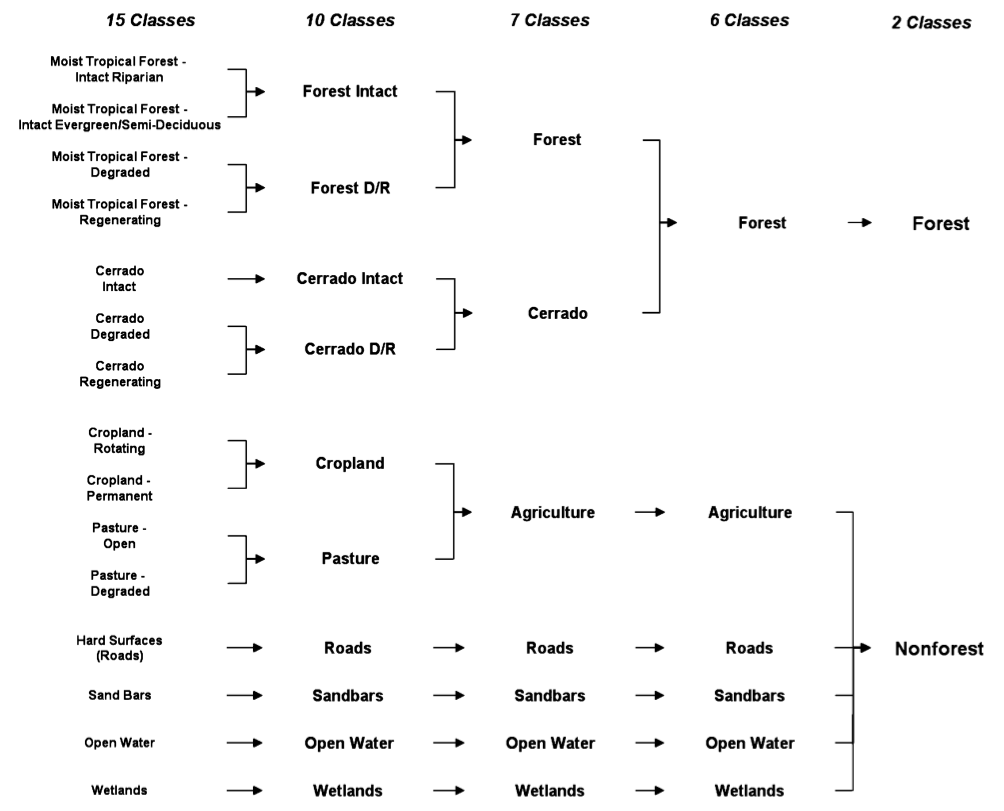
\includegraphics[width=1.0\textwidth]{fig_walker-hierarchy.png}
	\caption[Multi-level hierarchical classification system.]{Multi-level hierarchical classification system adopted by Walker et al. \citeyearpar{walker_large-area_2010}.}
	\label{fig: litrev-fig2.1}
\end{figure}

Currently, one of the most comprehensive, flexible, and internationally applied framework for land cover characterisation is the United Nations (UN) Land Cover Classification System (LCCS) developed by FAO (\cite{giri_brief_2012}). The UN LCCS was developed in response to a need for reliable, harmonised, and standardised information on land cover and land cover change (\cite{di_gregorio_land_2005}). It provides descriptors of land cover classes through a dichotomous, modular, hierarchical system for translation between typologies (\cite{defourny_revisiting_2012}) such that the comparison of land cover products, including qualitative and quantitative evaluations of product differences, are enabled (\cite{kuenzer_comparing_2014}). The first fully operational version of the UN LCCS was developed initially for the implementation of the AFRICOVER project (\cite{kalensky_africover_1998}; \cite{herold_evaluating_2012}). Some global land cover products that are compliant with the UN LCCS standards include the GLC2000 (\cite{bartholome_glc2000:_2005}) and GlobCover (\cite{arino_globcover:_2007}).

Two studies described as follows used PALSAR data for FAO LCCS-compliant land and forest cover mapping. Hoekman et al. \citeyearpar{hoekman_palsar_2010} mapped forest and land cover types in sub-continental Borneo using single- and dual-polarised PALSAR data in 2007. The resulting demonstration product was 85.5\% in full agreement with an independent reference dataset. The map legend consisted of 22 classes, including eight forest types, namely: tropical lowland forest, broadleaved evergreen; tropical mountain forest, broadleaved evergreen; riverine forest; swamp forest; mangrove forest; nipah mangrove forest; peat swamp (pole) forest; peat swamp (\textit{padang}) forest; and forest mosaics/fragmented or degraded forest. Except for nipah mangrove forest, the degree of full agreement was very high for lowland forest and fair/good for other natural forest types.

Another study by Otukei et al. \citeyearpar{otukei_using_2014} mapped land cover types in Bwindi Impenetrable National Park, Uganda based on the FAO Africover LCCS using quad- polarimetric ALOS/PALSAR data. The legend consisted of eight land cover types including dense evergreen forest, dry bare farmland, wet bare farmland, mixed farmland, mixed rangeland, degraded wetland, aquatic vegetation, and open water. An overall classification accuracy of 86\% was achieved, of which mixed rangeland and farmland were found to be the least discriminated.

While these studies and implementations, including the FAO GFRA-based land cover/forest type classification (see Appendix \ref{tab: appendix-table.a1}), applied hierarchically structured classification approaches, the determination of the sequence and order of the classes in these hierarchies were heuristically determined based on expert knowledge or on what made logical sense (i.e., similar to the \enquote{classification logic} proposed by Running et al. \citeyearpar{running_remote_1995} and implemented by DeFries et al. \citeyearpar{defries_global_1998} and Hansen et al. \citeyearpar{hansen_global_2000} for generating AVHRR-based global land cover products). For this study, a hierarchical clustering analysis was implemented (described in more detail in the next section) to determine a natural hierarchy of forest cover classes based on the multi-year PALSAR data, which would then define the multi-level class hierarchy to guide the execution of the classification.

\section{Cluster analysis}
\label{sec: litrev-cluster-analysis}

Cluster analysis, or clustering, is the art of finding groups or structure in the data (\cite{kaufman_introduction_1990}). The purpose of cluster analysis is to group observations into clusters in such a way that observations in the same cluster are more similar to one another than they are to observations in other clusters (\cite{bajorski_statistics_2011}). Cluster analysis, also often called unsupervised learning, does not require prior information about the groupings of observations and is commonly employed for descriptive or exploratory purposes to better understand the structure of the data (\cite{bajorski_statistics_2011}).

To measure the degree of similarity or dissimilarity between observations, distances are computed on the basis of their proximity in two-dimensional space in such that the smaller the distance between observations represents greater similarity and larger distances as less similarity (\cite{hair_multivariate_2013}). Euclidean distance is the most commonly used measure of similarity between two observations (\cite{kaufman_introduction_1990}), which is essentially a measure of the length of a straight line drawn between two observations when shown graphically.

\begin{figure}
	\centering
	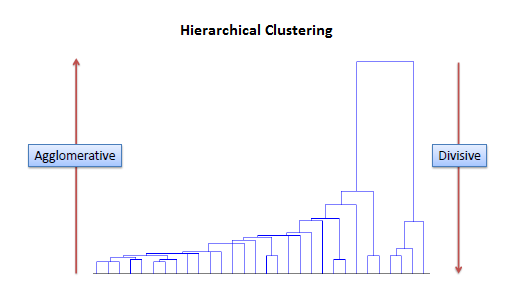
\includegraphics[width=1.0\textwidth]{fig_hierarchical-clustering.png}
	\caption[A dendrogram with arrows showing agglomerative and divisive hierarchical clustering techniques.]{A dendrogram with arrows showing agglomerative and divisive hierarchical clustering techniques (Source: Sayed, \citeyear{sayed_hierarchical_2016}).}
	\label{fig: litrev-fig2.2}
\end{figure}

There are two types of clustering procedures: hierarchical and non-hierarchical (or partitioning). Non-hierarchical clustering procedures divide the observations into a pre- defined number of clusters, which can be defined by the user or calculated within the algorithm (\cite{bajorski_statistics_2011}). The K-means is one of the most commonly used algorithms for non-hierarchical methods, which works by partitioning observations into a specified number of clusters and iteratively reassigns observations until a criteria for cluster homogeneity is met (\cite{hair_multivariate_2013}).

Hierarchical clustering procedures, on the other hand, do not require observations into a pre-defined number of clusters. The result is a tree structure, more commonly known as a dendrogram (see Fig. \ref{fig: litrev-fig2.2}), which is a graphical representation of the results of the hierarchical procedure that shows how the clusters are combined at each step of the procedure until all are contained in a single cluster (Hair et al., 2013). The dendrogram is a one-dimensional display of similarity with the height of the join indicating dissimilarity (\cite{ripley_pattern_1996}). According to Bajorski \citeyearpar{bajorski_statistics_2011}, hierarchical clustering methods often provide more clustering information than other methods.

Johnson \citeyearpar{johnson_hierarchical_1967} provided a succinct outline of the hierarchical clustering process. Given a dataset of N observations to be clustered and NxN distance (or similarity) matrix:

\begin{enumerate}
	\item Assign each observation to its own cluster, i.e., N observations will be equal to N clusters. Let the distances (or similarities) between clusters equal the distances similarities between observations they contain;
	\item Search for the closest (most similar) pair of clusters and combine them into a single cluster, such that there is one less cluster;
	\item Compute the distances (similarities) between the new cluster and each of the old clusters;
	\item Repeat steps \#2 and \#3 until all items are grouped into a single cluster of size N.
\end{enumerate}

In hierarchical clustering procedures, there are two types of methods: agglomerative and divisive (\cite{kaufman_introduction_1990}). These two methods construct their hierarchy in opposite directions (Fig. \ref{fig: litrev-fig2.2}). Divisive methods begin with all observations under one cluster and subsequently divide the data into the two meaningful clusters, then the process continues until the number of clusters is achieved. Agglomerative methods start with each observation forming a separate cluster, and are subsequently merged into the most similar clusters until all observations are in a single cluster.

The algorithm used in a hierarchical clustering procedure defines how similarity is measured in the clustering process (\cite{hair_multivariate_2013}). There are numerous algorithms for agglomerative methods, which only vary in their definition of between-cluster dissimilarity (\cite{kaufman_introduction_1990}). Some of the most common methods include (\ref{fig: litrev-fig2.3}): single linkage, complete linkage, and average linkage, which are described as follows (\cite{podani_introduction_2000}; \cite{bajorski_statistics_2011}; \cite{hair_multivariate_2013}):

\begin{itemize}
	\item Single linkage algorithm (also called minimum distance or nearest neighbor algorithm) defines similarity as the distance between the two closest elements between two clusters;
	\item Complete linkage algorithm (also called maximum distance or farthest neighbor algorithm) defines similarity as the distance between the two farthest elements from the two clusters; and
	\item Average linkage algorithm (also called average distance or unweighted pair-group average method) defines similarity as the average distance over all possible pairs of elements from the two clusters. The average linkage method gives a more robust solution compared to the two other techniques (\cite{sokal_principles_1963}; \cite{johnson_hierarchical_1967}).
\end{itemize}

\begin{figure}[!ht] \centering
	\captionsetup[subfigure]{width=2.0in} % <-- Use this to control text which is poorly spaced under a subfigure. 
	\begin{subfigure}[t]{0.32\textwidth}
		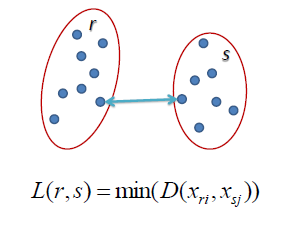
\includegraphics[width=\textwidth]{fig_clustering-single.png}
		\caption[Linkage methods in clustering.]{}
		\label{fig: litrev-fig2.3a}
	\end{subfigure}
	\begin{subfigure}[t]{0.32\textwidth}
		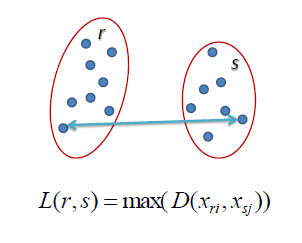
\includegraphics[width=\textwidth]{fig_clustering-complete.png}
		\caption[Linkage methods in clustering.]{}
		\label{fig: litrev-fig2.3b}
	\end{subfigure}
	\begin{subfigure}[t]{0.32\textwidth}
		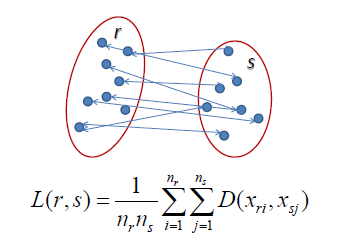
\includegraphics[width=\textwidth]{fig_clustering-average.png}
		\caption[Linkage methods in clustering.]{}
		\label{fig: litrev-fig2.3c}
	\end{subfigure}
	\caption[Methods for computing the distance matrix: (a) single linkage; (b) complete linkage; (c) average linkage.]{Methods for computing the distance matrix: (a) single linkage; (b) complete linkage; (c) average linkage (Source: Sayed, 2016).}
	\label{fig: litrev-fig2.3}
\end{figure}

In Fig. \ref{fig: litrev-fig2.3}, \textit{x} pertains to a set of objects within clusters \textit{r} and \textit{s}, of which \textit{L} is the distance between two clusters that may be defined as the shortest (single) or longest (complete) distance between two points in each cluster, or the average distance between each point in n number of points in one cluster to every point in the other cluster. A distance matrix \textit{D} is calculated where the \textit{i}th row and \textit{j}th column is the distance between the \textit{i}th and \textit{j}th elements.

Hierarchical clustering approaches to data classification are well-established in the biological sciences (i.e., numerical taxonomy) and the humanities (e.g., sociology, psychology), of which the common application is classification according to the relationships among the data observations being clustered (\cite{kaufman_introduction_1990}; \cite{podani_introduction_2000}).

In this study, a hierarchical agglomerative clustering procedure was implemented to determine and visualise the \enquote{natural} hierarchical structure of forest types based on the data with the aim of defining the forest classification hierarchy in contrast to the heuristic approaches such as those implemented by Pierce et al. \citeyearpar{pierce_knowledge-based_1994} and Dobson et al. \citeyearpar{dobson_knowledge-based_1996} to define classification hierarchies. The dendrograms from the cluster analyses were also compared to assess temporal consistency of the multi-year PALSAR mosaics.

\section{Decision tree classification}
\label{sec: litrev-decision-tree}

Classification of SAR data using traditional statistical techniques makes use of the unique local statistics of each image, which in turn necessitates local training and validation of each image; hence limiting its application at regional or global scales (\cite{dobson_knowledge-based_1996}). Knowledge-based or decision tree approaches were found to be more suitable for classifying SAR data (\cite{pierce_knowledge-based_1994}; \cite{dobson_knowledge-based_1996}). This is because decision tree classifiers apply hierarchical decision rules to differentiate land cover classes, and these decision rules or classifiers, once trained, become applicable to other images irrespective of scale and time (\cite{dobson_knowledge-based_1996}).

The decision tree algorithm, or classification and regression trees (CART), is based on the seminal work of Breiman et al. \citeyearpar{breiman_classification_1984}. The decision tree classifier is a simple, non-parametric, binary recursive partitioning procedure in the form of hierarchical rules that are successively applied to the input data or feature space (\cite{strobl_introduction_2009}). The goal of the recursive partitioning is to use a set of predictor variables to estimate the means of one or more response variables; thereby constructing a nested binary tree from the repeated splitting of the data into homogenous subsets (\cite{michaelsen_regression_1994}). The full dataset (parent node) is partitioned into two groups based on a single predictor variable. Each resulting subset (child node) is further partitioned such that the variability in the response variables are minimised and the nodes contain more homogenous observations (\cite{berk_classification_2008}). Once partitioning is complete, the means of the response variables in each terminal node serve as rules for predicting future observations (\cite{michaelsen_regression_1994}; \cite{berk_classification_2008}; \cite{strobl_introduction_2009}).

Decision trees can grow to their maximum size since the splitting of each node continues recursively without a stopping criterion, and eventually the process stops until no further splits are possible due to lack of data (\cite{wu_top_2009}). Larger decision trees have fewer classification errors, hence less bias, but have terminal nodes with few observations, hence greater variance and instability (\cite{berk_classification_2008}). A pruning sequence is then implemented to find a sensible trade-off. Pruning, a process aimed at constraining the size of the tree to avoid overfitting the data, involves removing inefficient branches of the decision tree by consolidating nodes that do not reduce heterogeneity despite the added extra tree complexity (\cite{berk_classification_2008}; \cite{strobl_introduction_2009}). An optimal tree is identified by evaluating the predictive performance of every tree in the pruning sequence either on independent test data or through cross-validation (\cite{wu_top_2009}). Cross-validation, as implemented in this study, involves partitioning the full dataset into subsets, excluding one subset, growing the tree on the remaining data, and testing it on the excluded subset (\cite{michaelsen_regression_1994}). The chances of overfitting is minimised since essentially different data are used to train and test the decision trees.

Several examples have successfully demonstrated the use of decision tree classifiers for the classification of remotely sensed data. With optical data, decision trees have been used for generating global land cover classification map products from the AVHRR sensor (\cite{defries_global_1998}; \cite{hansen_global_2000}); for mapping land and forest cover change in Palawan and Eastern Mindanao in the Philippines from Landsat data (\cite{pereira_forest_2006}); and for mapping decadal mangrove cover change in the Philippines using Landsat (\cite{long_mapping_2013}), among others.

With SAR data, Simard et al. \citeyearpar{simard_use_2000} used decision trees and multi-scale texture measures on the Japan Earth Resources Satellite (JERS-1) SAR data for thematic mapping of tropical forest in Gabon in Central Africa, of which decision trees resulted in improving classification results. Both JERS-1 and the European Resources Satellite (ERS-1) SAR composites were used with a decision tree classifier for mapping land cover in Michigan in the United States (\cite{dobson_knowledge-based_1996}), and for mapping coastal vegetation in Gabon in Central Africa (\cite{simard_mapping_2002}). Dong et al. \citeyearpar{dong_50-m_2014} mapped broad land cover categories (i.e., forest, cropland, urban, water) in Southeast Asia using dual-polarised PALSAR data and a decision tree classifier, and achieved high overall accuracy. The producer's and user's accuracies of forest were 86\% and 93\%, which was partly attributed the simple classification scheme.

Decision trees have a number of advantages over traditional classification methods. Hansen et al. \citeyearpar{hansen_classification_1996} showed that decision trees slightly outperformed maximum likelihood algorithm for classifying monthly composites of AVHRR data. Moreover, decision trees provided an added advantage of reducing data dimensionality by revealing the hierarchical nature of predictor variables, specifically those metrics that contributed to discriminating among cover types. Friedl \& Brodley \citeyearpar{friedl_decision_1997} found that decision tree algorithms consistently outperformed the maximum likelihood and linear discriminant classifiers in terms of classification accuracies applied to global AVHRR data. Pal \& Mather \citeyearpar{pal_assessment_2003} showed that decision trees when applied to Landsat and hyperspectral data performed acceptably well compared to the maximum likelihood and artificial neural network classifiers, except with high-dimensional data. Otukei \& Blaschke \citeyearpar{otukei_land_2010} found that decision trees performed better than maximum likelihood and support vector machines for land cover change assessment using Landsat data. Mishra et al. \citeyearpar{mishra_land_2011} evaluated different classification algorithms for classifying land cover using fully polarimetric ALOS/PALSAR data, and found that decision trees produced more accurate results than parallelepiped, minimum distance, maximum likelihood, and Wishart classifiers.

In this study, a decision tree classifier was used similarly due to its better performance over other classification algorithms, its suitability for classifying SAR data, and its potential applicability of decision rules to images over other areas once the classifier has been trained.

\section{Texture: the grey-level co-occurrence matrices}
\label{sec: litrev-texture-glcm}

Image texture refers to the spatial variability or the patterns of spatial relationships of grey levels (tone) within a neighbourhood of pixels, which is commonly described in terms of roughness or smoothness (Mather \& Koch, 2011). Texture is one of the important elements of image interpretation that are used to describe the characteristics of features in remotely sensed images (Campbell \& Wynne, 2011).

Previous research have utilised different texture information with SAR data for various aspects of land and forest cover type mapping such as improving the discrimination of forest types (Ulaby et al., 1986); detecting clearings in primary forest (Oliver, 2000); discriminating different subcategories of forest vegetation types (Saatchi et al., 2000); mapping of tropical forest (Simard et al., 2000); discriminating inundated vegetation (Podest \& Saatchi, 2002); increasing the accuracy of biomass estimation in tropical forests (Kuplich et al., 2005); and improving the classification accuracies of broad land cover types (Walker et al., 2010; Longépé et al., 2011; Li et al., 2012; Rakwatin et al., 2012).

First- and second-order texture measures are among the descriptors that can be measured in an image. First-order texture measures calculate the spectral variability or statistical moments (e.g., mean, variance, kurtosis, skewness) within a certain window (group of pixels or kernel), of which the moments do not contain any direction (Kurvonen \& Hallikainen, 1999). Second-order texture measures consider the spatial relationships between groups of two neighboring pixels to a certain direction within the window (Gallardo-Cruz et al., 2012). The calculation of second-order texture measures involves the construction of Grey-Level Co-occurrence Matrices (GLCM), which are matrices containing the probabilities of co-occurrence of pixel values for pairs of pixels in a given direction and distance (Gallardo-Cruz et al., 2012).

\begin{figure}
	\centering
	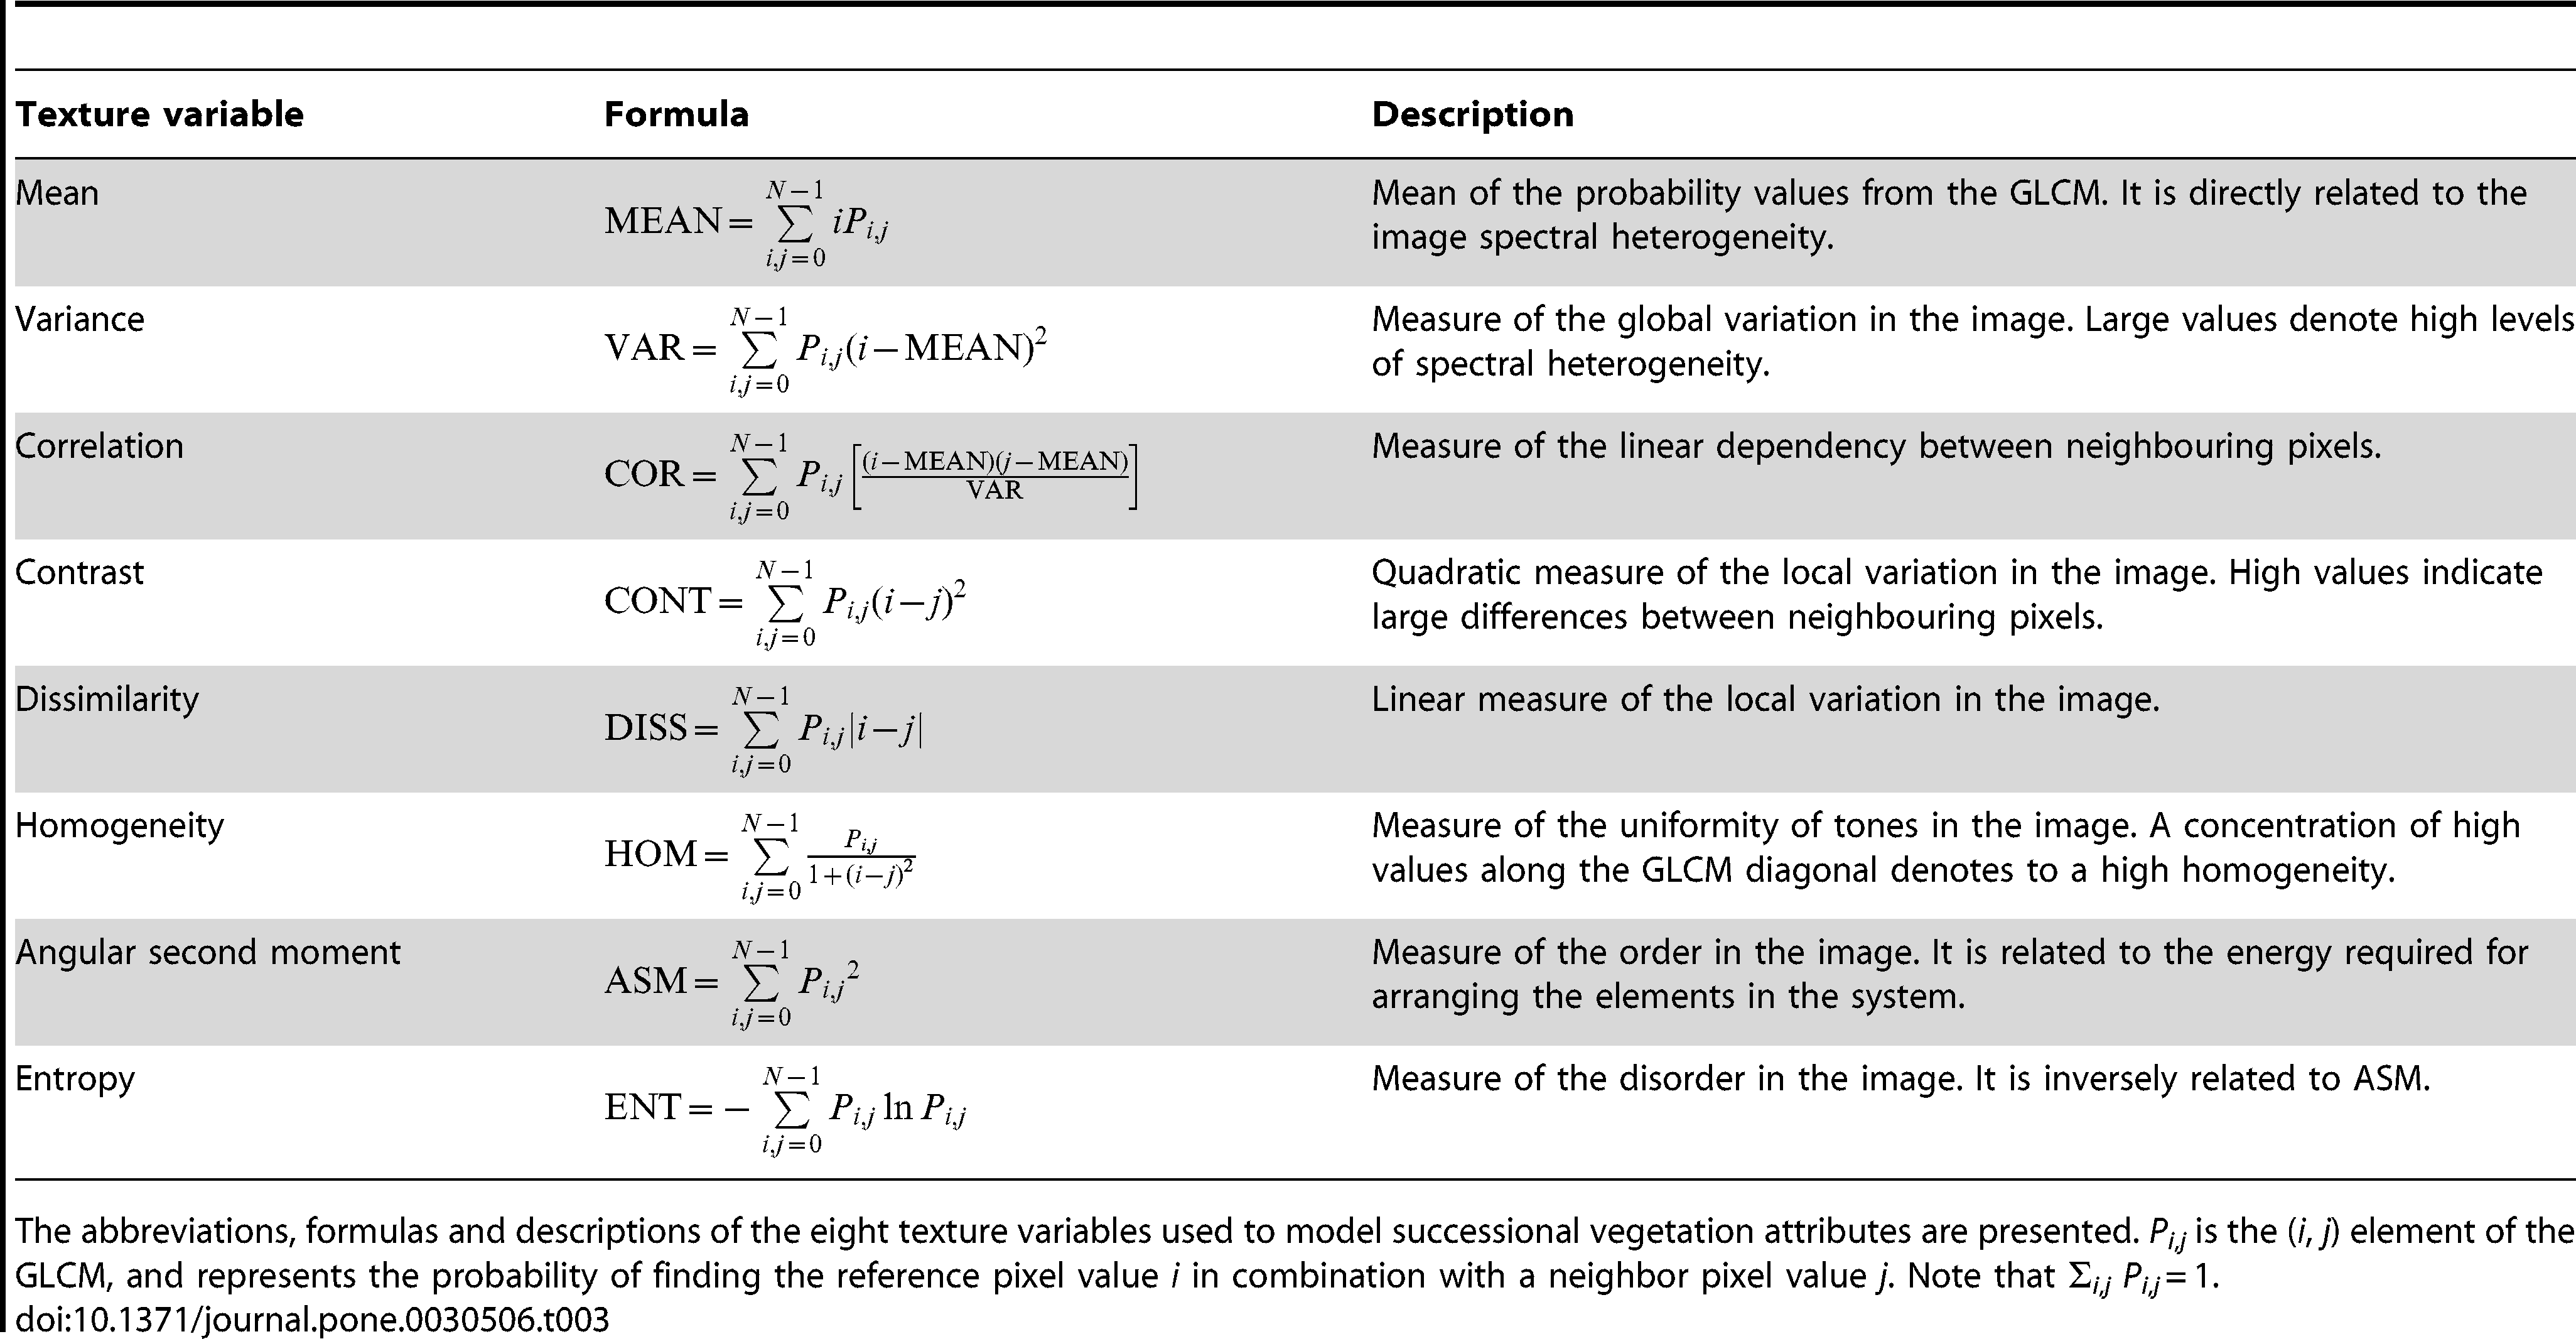
\includegraphics[width=1.0\textwidth]{fig_texture-measures.png}
	\caption[Texture variables derived from the grey-level co-occurrence matrix.]{Texture variables derived from the grey-level co-occurrence matrix (Source: Gallardo-Cruz et al., 2012).}
	\label{fig: litrev-fig2.4}
\end{figure}

The GLCM, a concept first described by Haralick et al. (1973), outlines the distance and angular relationships among a neighbourhood of pixels. It computes the joint probability of occurrence \textit{p(i,j)} of the pairs of grey levels i and j separated by a given distance dij and direction, and the image being initially quantised into \textit{N\textsubscript{g}} grey levels (Haralick et al., 1973). In this study, eight texture variables in three groups were used to describe the degree of contrast between pixels (contrast, dissimilarity, homogeneity), the regularity in the pixels within a neighbourhood of pixels (angular second moment, entropy), and the statistics derived from the GLCM (mean, correlation, variance) (Fig. \ref{fig: litrev-fig2.4}; Gallardo-Cruz et al., 2012).\\

In this study, the texture measures listed in Fig. \ref{fig: litrev-fig2.4}, in addition to radar backscatter and topographic variables, were evaluated whether they contributed to improving the classification and discrimination of forest cover types based on the FAO forest classification.

\section{Geographic object-based image analysis}
\label{sec: litrev-geobia}

Geographic Object-Based Image Analysis (GEOBIA) is a recent sub-discipline of geographic information science (including its own theory, methods, and tools) that intends to develop automated approaches to partition remote sensing imagery into meaningful image-objects, and assess their characteristics through spatial, spectral, and temporal scales (Hay \& Castilla, 2008). Its main objective is to generate new geographic information (in GIS-ready format) from which spatial knowledge can be obtained (Blaschke et al., 2014). It serves as a critical bridge to the raster (remote sensing) and vector (GIS) domains through the generation of image-objects, which represent meaningful geographic entities that can be distinguished in an image. Fundamentally, GEOBIA consists of image segmentation, classification of objects, and modeling based on characteristics of objects (Johansen et al., 2010).

Object-based approaches were developed to address the limitations of traditional pixel-based approaches for image analysis, classification, and interpretation. Burnett \& Blaschke (2003) argued that pixel-based methods do not maximise the use of the spatial concepts of neighbourhood, proximity, or homogeneity for characterising land use/land cover using remotely sensed data. The pixel-centered approach, which adheres to the concept of the pixel as a spatial entity (Fisher, 1997), assumes the pixel to be equivalent to objects in the landscape (Burnett \& Blaschke, 2003). Wu (1999) suggested that the hierarchical patch dynamics framework can be used model landscapes as a hierarchical mosaic of patches such that ecological systems can be recognised as spatially nested patch hierarchies, wherein larger patches are composed of smaller patches. In simple terms, an image composed of pixels is partitioned into segments (or patches), and groups of related segments form larger segments (e.g., individual tree segments combine to form a forest segment).

In its broadest sense, image segmentation refers to the process of partitioning an image, which is basically an array of measurements, into multiple spatially discrete regions on the basis of spectral homogeneity (Blaschke et al., 2014; Canty, 2014). It is the first step in a processing workflow to derive meaningful image-objects. Multi-scale segmentation or object relationship modelling, the method developed by Burnett \& Blaschke (2003) to derive meaningful objects from images, relies heavily on the hierarchical patch dynamics theory, image segmentation, and in defining the semantic rules to establish relationships of the lower landscape units to higher levels of organisation. Semantics based on descriptive assessment and knowledge is used in GEOBIA to translate spectral characteristics of image-objects to real-world features, such that groups of pixels are now put into context (Blaschke et al., 2014).

Object-based approaches have been used for land and forest cover mapping and characterisation, specifically using SAR data. Some examples of these applications include delineation of forest cover maps and detection of deforestation in Europe (Thiel et al., 2008); mapping changes in the largest continuous Amazonian mangrove belt (Nascimento et al., 2013); mapping mangroves in Guinea, West Africa (Flores De Santiago et al., 2013); and classifying wetland vegetation types (Hong et al., 2015). In some of these studies, implementing an object-based approach allowed the inclusion of other data sources such as digital elevation models (DEM) or texture measures, in addition to the SAR images themselves, to provide more information in aid of image analysis, classification, and interpretation. Others studies also combined of multi-sensor and multi-temporal SAR data such as for mapping land cover and seasonal inundation in the Brazilian Pantanal Wetland by using L-band ALOS/PALSAR and C-band RADARSAT-2 data (Evans et al., 2010; Evans \& Costa, 2013; Evans et al., 2014).

A notable example that is useful for this present study is the paper by Walker et al. (2010), which compared the performance of Landsat and ALOS/PALSAR for large-area land and forest cover classification and mapping in the Brazilian Amazon. They designed an object-based image analysis approach combining imagery with information from elevation layers and feature extraction, and applied a decision tree classifier within the context of a hierarchical, multi-level classification scheme. Their study confirmed the potential of ALOS/PALSAR as an accurate source for spatially explicit estimates of forest cover, and pointed to the important role of spaceborne radar sensors in complementing optical remote sensing for forest cover mapping and monitoring.

For this study, an object-based approach was implemented, in contrast to traditional pixel-based approaches, since previous research have applied this on SAR data for forest cover mapping with better results and classification accuracies. One advantage of an object-based approach over a pixel-based approach is the inclusion of ancillary datasets to improve the analysis and classification of remotely sensed data. For example, topographic data, such as elevation and slope, can be included to complement dual- polarised ALOS/PALSAR mosaic data to provide additional information that can aid in land and forest cover classification and mapping since topography influences forest typology.

\section{Conceptual framework}
\label{sec: litrev-conceptual-framework}

This study is about the evaluation of multi-year ALOS/PALSAR mosaic data for mapping and monitoring of forest cover types in the Philippines. The conceptual framework of this study presents Forest as the central theme and the utilisation of remote sensing data and techniques for forest applications (Fig. \ref{fig: litrev-fig2.5}). The four main elements of the study consist of Data, Method, Indicator, and Application. Data elements consist of SAR, DEM, and ancillary land cover maps. Method elements include FCCS, GEOBIA, GLCM, clustering, and CART. Indicator elements include consistency, hierarchy, and accuracy. Application elements consist of mapping, classification, and monitoring.

The Data-Method relationship describes the dataset as inputs to the methodology and the suite of methods implemented on the data. The Method-Indicator relationship describes the methodology for exploring these indicators and the indicators provide a measure of the efficacy of the methods in producing the intended result. The Indicator-Application relationship describes the quality of these indicators for the intended applications and the applications provide feedback to these indicators over time. The Data-Application describes the use of the data for the intended applications, of which in turn also provide feedback on the applicability and utility of the data for the intended purpose.

\begin{figure}
	\centering
	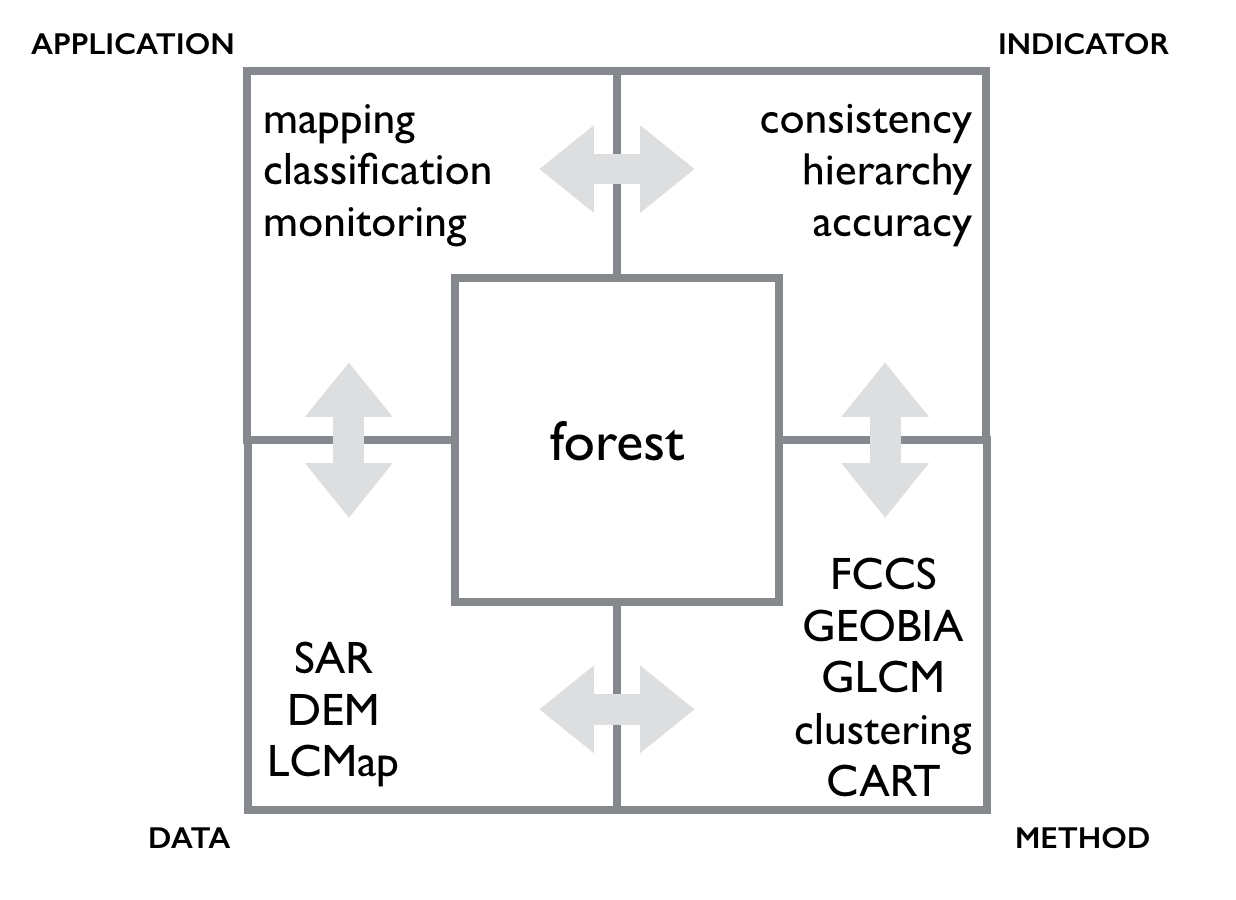
\includegraphics[width=1.0\textwidth]{fig_conceptual-framework.png}
	\caption[The conceptual framework of the study shows forest as the central theme enclosed by elements concerning data, method, indicator, and application, and their interrelationships.]{The conceptual framework of the study shows forest as the central theme enclosed by elements concerning data, method, indicator, and application, and their interrelationships.}
	\label{fig: litrev-fig2.5}
\end{figure}

\section{Aims and objectives}
\label{sec: litrev-aims-objectives}

Given the capabilities of ALOS/PALSAR data and above-mentioned image processing techniques, it is worth exploring their potentials for land and forest cover mapping in the Philippines. The general aim of this master’s research is to evaluate the suitability of ALOS/PALSAR mosaic data for mapping and monitoring of forest cover types in the Philippines based on the FAO forest cover classification system. To achieve this, the specific objectives of this thesis are as follows:

\begin{enumerate}
	\item To ascertain whether ALOS/PALSAR mosaic data are temporally consistent within a single acquisition year and across multiple acquisition years for the purpose of periodic monitoring;
	\item To establish a forest classification hierarchy based on the FAO forest classification system, and assess its consistency temporally and across feature attributes;
	\item To assess discrimination of forest cover types using ALOS/PALSAR mosaic data based on polarisation, topographic, and texture characteristics;
	\item To determine whether ancillary feature attributes (i.e., topographic, texture), in addition to polarisation, contribute to improving the classification accuracy of forest cover types; and
	\item To develop a hierarchical, stepwise classification approach for assessing the degree at which ALOS/PALSAR mosaic data can discriminate between forest cover types.
\end{enumerate}

\section{Scope and limitations}
\label{sec: litrev-scope-limitations}

Reference data used for this study, particularly as training and validation for the image classification, does not make use of ground-truth data. Rather, the study made use of the 2010 NAMRIA land cover map as the reference data. The official land cover map product was validated in the field by NAMRIA and fulfills acceptable classification accuracies (Raul Magabo, 2015, \textit{personal communication}), although documentation of the methods and accuracy assessment to accompany the map product has not yet been made publicly available. The multi-year ALOS/PALSAR mosaic data used in this study, which are different from the standard strip data product, were accessed through JAXA's Kyoto \& Carbon (K\&C) Initiative and were provided as is. The findings from this study may apply to the standard products, but may potentially differ unless the same pre- processing steps carried out on the mosaic data (Shimada \& Ohtaki, 2010) are similarly applied on the standard products.
